%%% Fun stuff:
%\footnote{NGC 2146 - ESA/Hubble \& NASA}
%
%\begin{itemize}
%\item Item 1 
%\item Item 2
%\end{itemize}
%
%\begin{figure}
%\fbox{\includegraphics[width=8cm]{figure.jpg}}
%\end{figure}
%
%\center{\alert{Bright Red Text}}
%
%\begin{block}{Text above the block}
%\begin{figure}
%\includegraphics[width=9cm]{figure.jpb}
%\end{figure}
%\end{block}
%
%\uncover<2>{This text will show up on the second slide.}
%
%\invisible<2>{This text will be invisible on the second slide.}
%
%\begin{columns}[c]
%\column{.6 \textwidth}
%First column text
%\begin{itemize}
%\item Item 1
%\end{itemize}
%\column{.2 \textwidth}
%Second column text
%\end{columns}

\documentclass[blue,serif]{beamer}


\usepackage{datetime}
\usepackage[dark]{beamerthemesidebar}
\usepackage[english]{babel}
\usepackage{graphicx}
\usepackage{amsmath}
\usepackage{amssymb}
%\usepackage[dvipsnames]{xcolor}
\usepackage{xcolor}
%\usepackage[latin1]{inputenc}
%\renewcommand{\thefootnote}{}
\usepackage{times}
\usepackage[T1]{fontenc}
\beamertemplatenavigationsymbolsempty

\setbeamertemplate{enumerate item}{(\alph{enumi})}
\setbeamertemplate{enumerate subitem}{(\roman{enumii})}

\def\be{\begin{equation*}}
\def\ee{\end{equation*}}
\def\bea{\begin{eqnarray*}}
\def\eea{\end{eqnarray*}}

\title[Side Deck - Capsone 1]
      {Side Deck - Capstone 1}

\subject{Side Deck - Capstone 1}

\begin{document}

\addtobeamertemplate{footline}{
  \setlength\unitlength{1ex}
  \begin{picture}(0,0) 
    % \put{} defines the position of the frame
    \put(0,0){\makebox(0,0)[bl]{
    
\includegraphics[width=2.5cm]{figures/springboard logo-1.png}
   % \includegraphics{figures/image2.png}
 %   \includegraphics{figures/image3.png}
    }}
  \end{picture}%
}{}

%%%%%%%%%%%%%%%%%%%%%%%%%%%%%%
%%%%% Slides Start Here %%%%%%
%%%%%%%%%%%%%%%%%%%%%%%%%%%%%%

\begin{frame}{Rapid COVID-19 Diagnosis using Raman Spectroscopy and Machine Learning}

\begin{columns}[c]
\column{.6 \textwidth}
  \begin{figure}
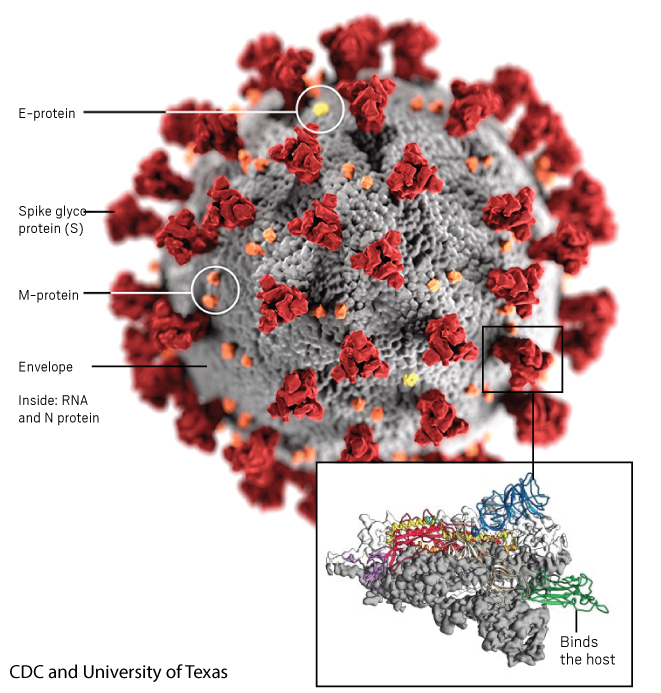
\includegraphics[width=5cm]{figures/covid_virus_logo.jpg}
 \end{figure}
  \vspace{-.4cm}
\column{.4\textwidth}
%  \textBig{Capstone 2 project presentation}
   \center{\textbf{Author:} Isaac Ghebregziabher} \vspace{-.1cm}
%   \center{\textbf{Supervisor:} Yuxian Xin}
%   \vspace{-.3cm}
    \center{Capstone Project One}
    \center{\today}
\end{columns}
%\center{Capstone Project One}
%\vspace{0.2cm}
%\vspace{-.3cm}


\end{frame}

%%%%%%%%%%%%%%%%%%%%%%%%%%%%%%
%%%%%%%%%%%%%%%%%%%%%%%%%%%%%%
\section{Introduction} %%%%
%%%%%%%%%%%%%%%%%%%%%%%%%%%%%%
%%%%%%%%%%%%%%%%%%%%%%%%%%%%%%

\begin{frame}{World under COVID-19 pandemic crisis}
%\linespread{1.3}

%\begin{columns}
%	\column{.6 \textwidth}
\begin{itemize}
   \item > 171 million active cases
	\item 3.5+ million deaths
	\item Fast and reliable diagnostic is needed
\end{itemize}

%	\column{.4 \textwidth}
	\begin{figure}
		
		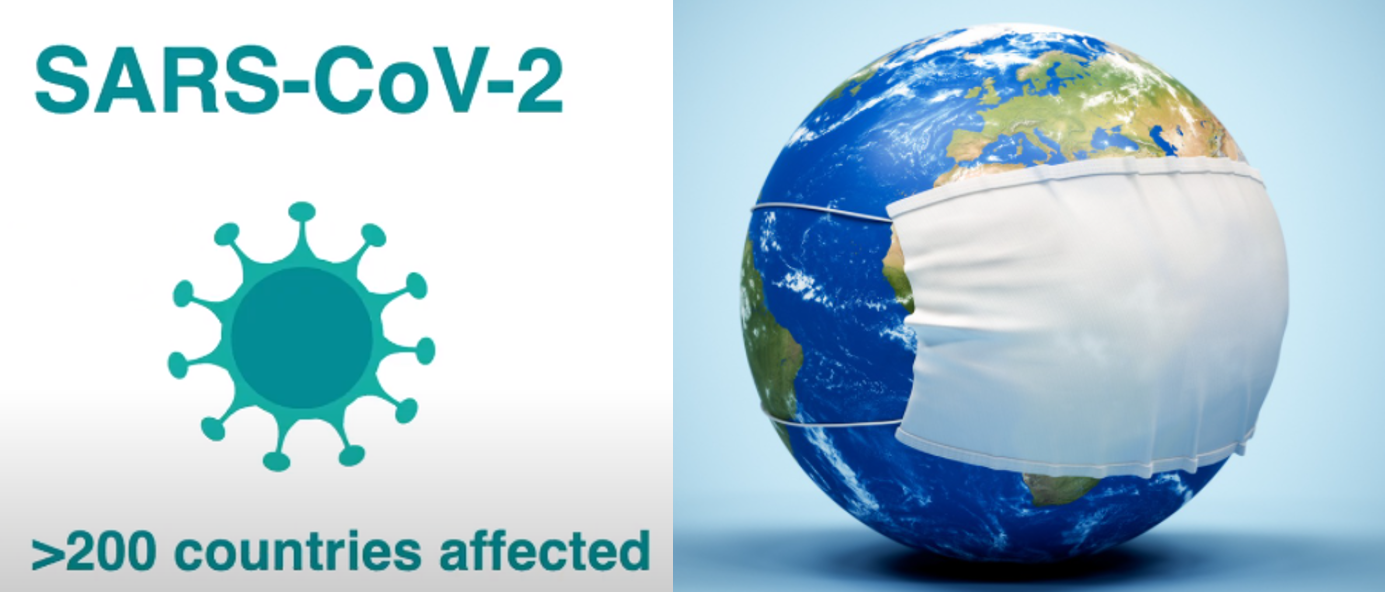
\includegraphics[width=9.0cm]{figures/raman_covid_intro.png}
%		\caption{Single valued features (dropped).}
	\end{figure}
%\end{columns}


\end{frame}

%%%%%%%%%%%%%%%%%%%%%%%%%%%%%%
%%%%%%%%%%%%%%%%%%%%%%%%%%%%%%
\section{Current diagnostic method} %%%%
%%%%%%%%%%%%%%%%%%%%%%%%%%%%%%
%%%%%%%%%%%%%%%%%%%%%%%%%%%%%%

\begin{frame}{RT-PCR – Current COVID-19 detection method is time consuming and expensive}
%\linespread{1.3}

%\begin{columns}
%	\column{.6 \textwidth}
\begin{itemize}
   \item 3 days for sample preparation and RNA extraction
	\item Expensive PCR
%	\item Fast and reliable diagnostic is needed
\end{itemize}

%	\column{.4 \textwidth}
	\begin{figure}
		
		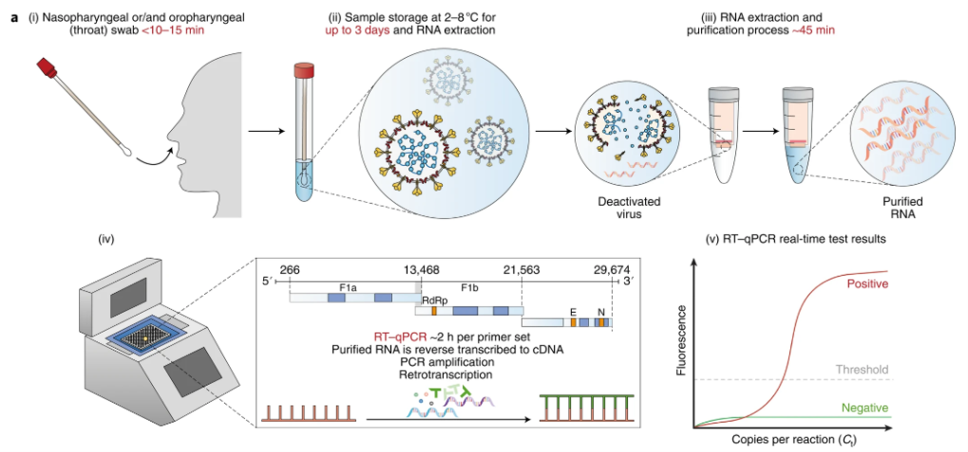
\includegraphics[width=9.0cm]{figures/raman_covid_RT_PCR.png}
%		\caption{Single valued features (dropped).}
	\end{figure}
%\end{columns}


\end{frame}

%%%%%%%%%%%%%%%%%%%%%%%%%%%%%%
%%%%%%%%%%%%%%%%%%%%%%%%%%%%%%
\section{Raman spectroscopy} %%%%
%%%%%%%%%%%%%%%%%%%%%%%%%%%%%%
%%%%%%%%%%%%%%%%%%%%%%%%%%%%%%

\begin{frame}{Principle of Raman effect}
%\linespread{1.3}

%\begin{columns}
%	\column{.6 \textwidth}
\begin{itemize}
   \item Most light scatters unaffected (Rayleigh scattering)
	\item A few percent gets Raman scattered
	\item Raman Scattered light is signature of molecular composition
%	\item Fast and reliable diagnostic is needed
\end{itemize}

%	\column{.4 \textwidth}
	\begin{figure}
		
		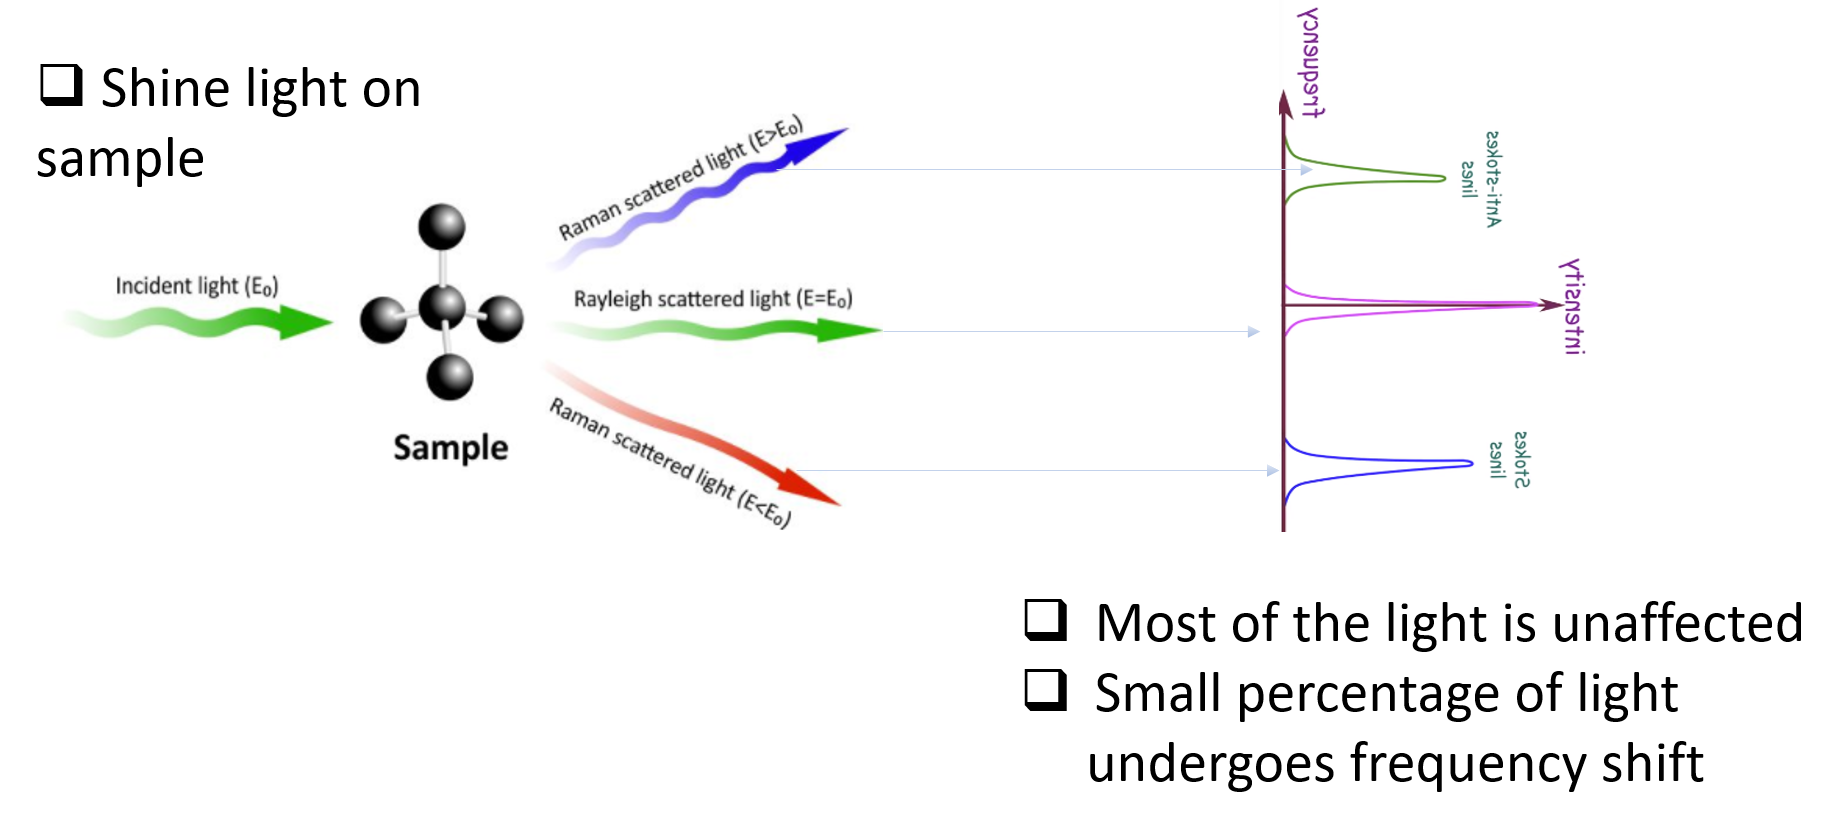
\includegraphics[width=9.0cm]{figures/raman_principle3.png}
%		\caption{Single valued features (dropped).}
	\end{figure}
%\end{columns}


\end{frame}

%%%%%%%%%%%%%%%%%%%%%%%%%%%%%%
%%%%%%%%%%%%%%%%%%%%%%%%%%%%%%
\subsection{Raman and ML} %%%%
%%%%%%%%%%%%%%%%%%%%%%%%%%%%%%
%%%%%%%%%%%%%%%%%%%%%%%%%%%%%%

\begin{frame}{Rapid detection of Covid-19 using Raman spectroscopy and Machine Learning}
%\linespread{1.3}

%\begin{columns}
%	\column{.6 \textwidth}
%\begin{itemize}
%   \item Most light scatters unaffected (Rayleigh scattering)
%	\item A few percent gets Raman scattered
%	\item Raman Scattered light is signature of molecular composition
%	\item Fast and reliable diagnostic is needed
%\end{itemize}

%	\column{.4 \textwidth}
	\begin{figure}
		
		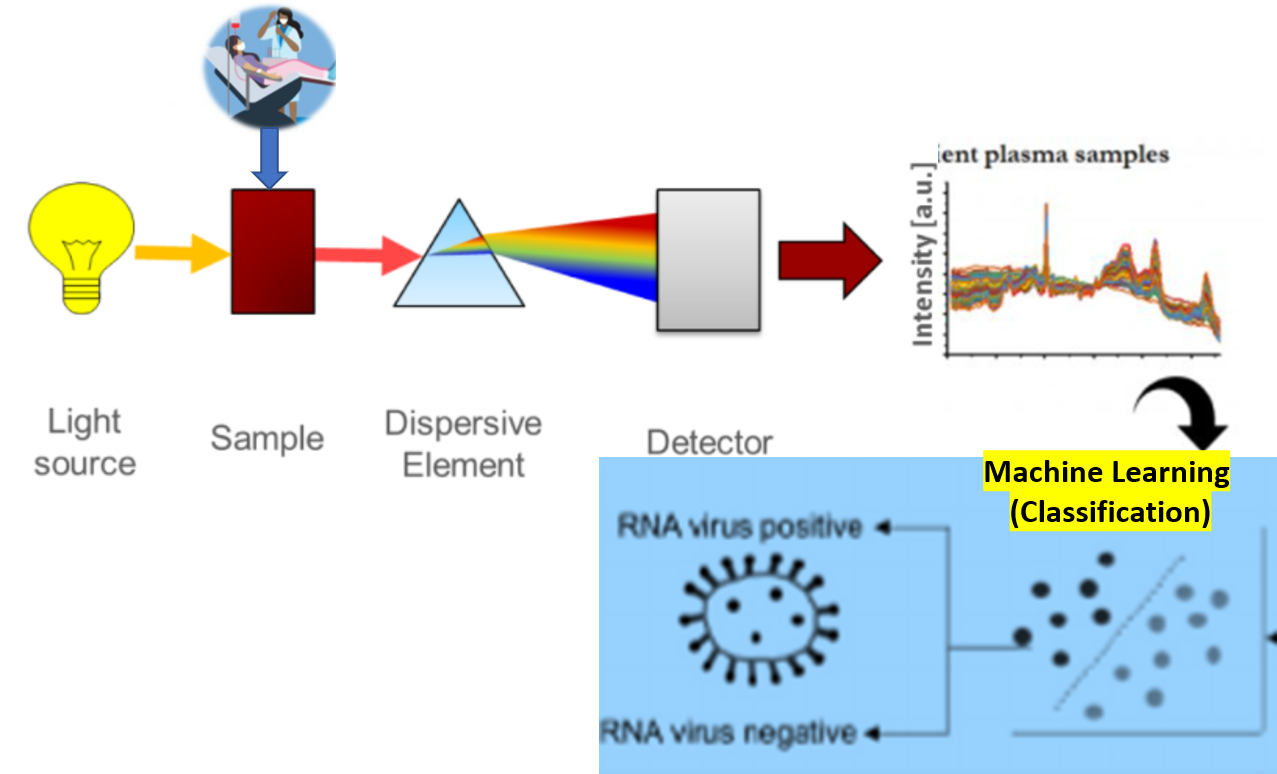
\includegraphics[width=9.0cm]{figures/covid_raman_and_ML.png}
%		\caption{Single valued features (dropped).}
	\end{figure}
%\end{columns}


\end{frame}


%%%%%%%%%%%%%%%%%%%%%%%%%%%%%%
%%%%%%%%%%%%%%%%%%%%%%%%%%%%%%
\section{Data Wrangling} %%%%
%%%%%%%%%%%%%%%%%%%%%%%%%%%%%%
%%%%%%%%%%%%%%%%%%%%%%%%%%%%%%

\begin{frame}{Overview of Dataset obtained from Kaggle}
%\linespread{1.3}

%\begin{columns}
%	\column{.6 \textwidth}
\begin{itemize}
    \item 309 rows X 901 columns
    \item Each column $\rightarrow$ Raman Wavenumber
	\item Rows $\rightarrow$ Intensity for wavenumbers
	\item Each row corresponds to one observation
	\item Last column `\textit{\textbf{diagnostic}}' is target variable
\end{itemize}

%	\column{.4 \textwidth}
	\begin{figure}
		
		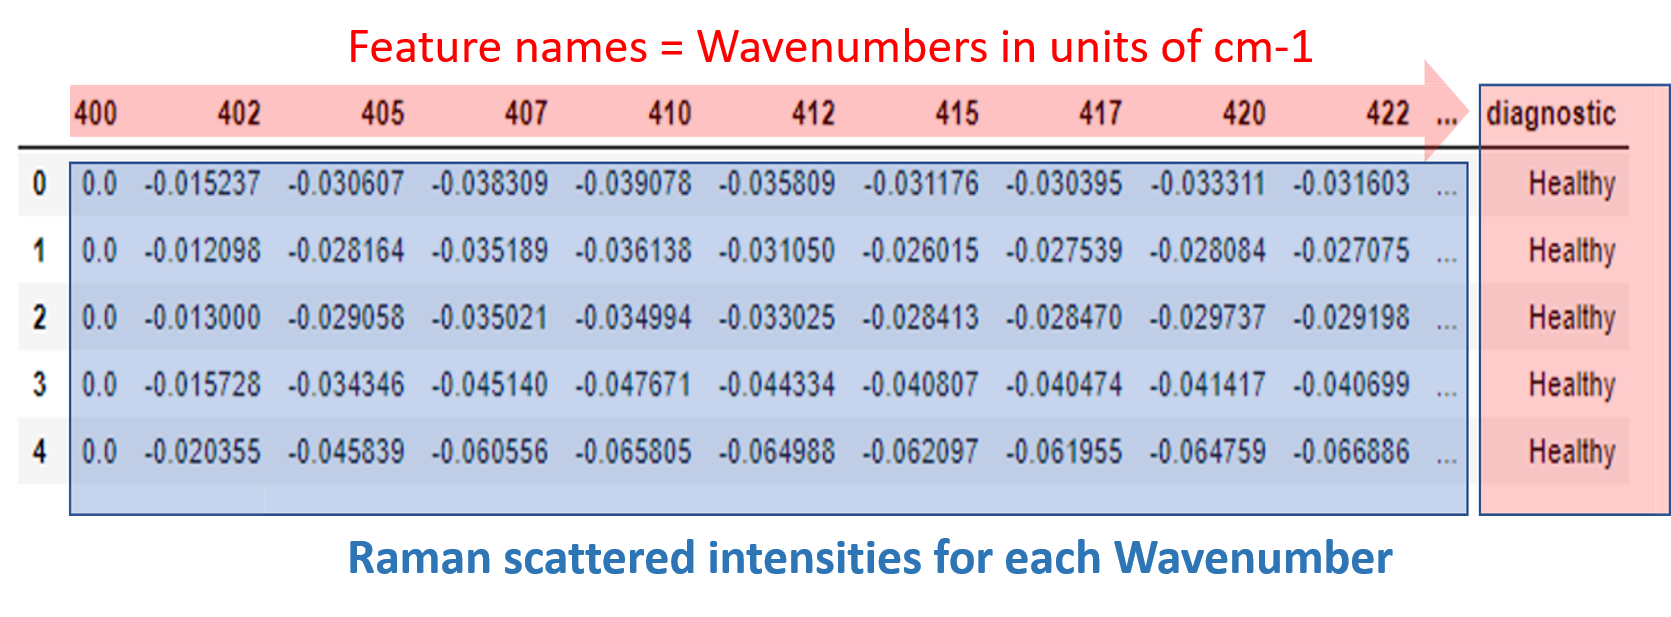
\includegraphics[width=8.0cm]{figures/raman_dataset.png}
%		\caption{Single valued features (dropped).}
	\end{figure}
%\end{columns}


\end{frame}

\begin{frame}{Raman detector might have dead pixels corresponding to all zero value intensities}
%\linespread{1.3}

%\begin{columns}
%	\column{.6 \textwidth}
\begin{itemize}
    \item No missing values in dataset
	\item 9 features wave-numbers with 0 intensity value
	\item Drop null features (treated as missing)
\end{itemize}

%	\column{.4 \textwidth}
	\begin{figure}
		
		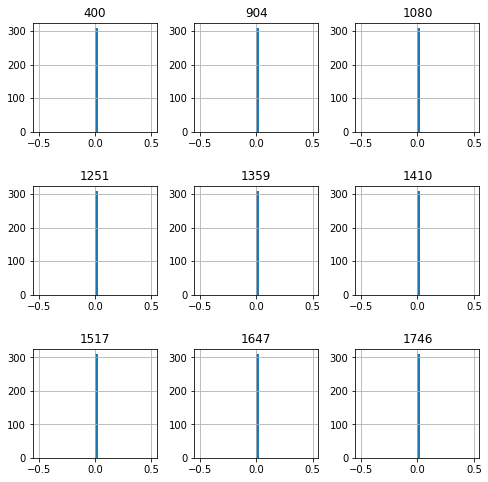
\includegraphics[width=5.0cm]{figures/dropped.png}
		\caption{Single valued features (dropped).}
	\end{figure}
%\end{columns}


\end{frame}

%\begin{frame}{Remaining features have normal distribution }
%\linespread{1.3}

%\begin{columns}
%	\column{.6 \textwidth}
%\begin{itemize}
%    \item No concern on feature distributions.
%	\item Most close to normal.
%	\item little skew on several features.
%\end{itemize}

%	\column{.4 \textwidth}
%	\begin{figure}
		
%		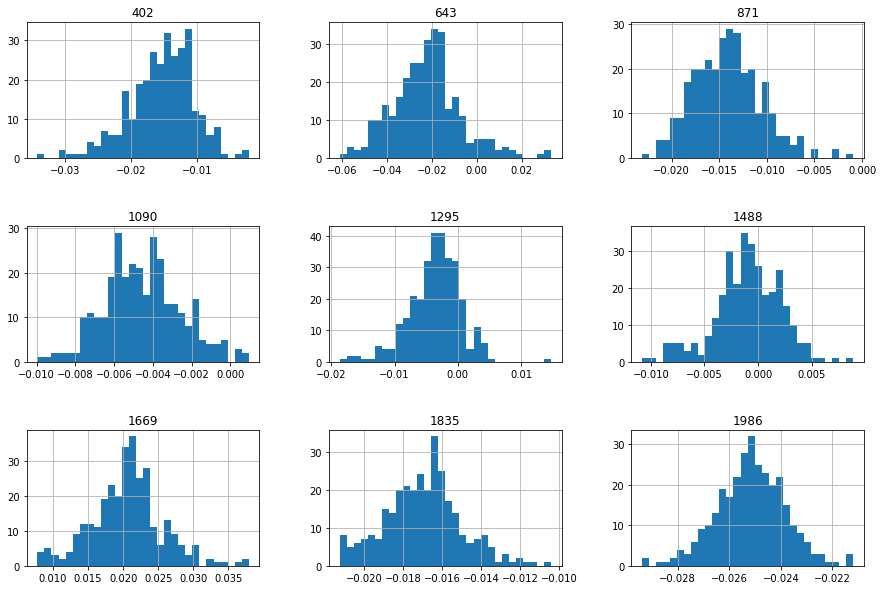
\includegraphics[width=5.0cm]{feature_normal.png}
%		\caption{Close to normal feature distributions.}
%	\end{figure}
%\end{columns}


%\end{frame}

%%%%%%%%%%%%%%%%%%%%%%%%%%%%%%
%%%%%%%%%%%%%%%%%%%%%%%%%%%%%%
\section{Exploratory Data Analysis} %%%%
%%%%%%%%%%%%%%%%%%%%%%%%%%%%%%
%%%%%%%%%%%%%%%%%%%%%%%%%%%%%%

\begin{frame}{Dataset is balanced}
%\linespread{1.3}
\begin{itemize}
    \item No class imbalance issues
    \item Dataset is balanced with $\approx$ 50:50 class ratio.
\end{itemize}
\begin{figure}
		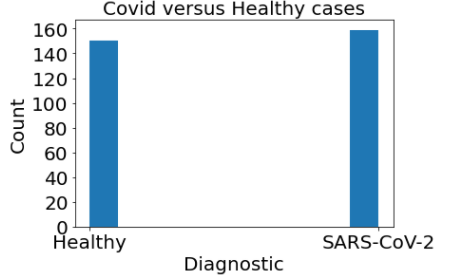
\includegraphics[width=7.0cm]{balance.png}
		\caption{$\approx 50:50$ COVID to Healthy class ratio.}
	\end{figure}

\end{frame}

\begin{frame}{Visually indiscernible Raman spectrum}
%\linespread{1.3}
\begin{itemize}
    \item Visually difficult to easily identify COVID from Healthy.
    \item Machine Learning model is needed for fast and reliable COVID diagnosis.
    %\item Dimension reduction with PCA
\end{itemize}
\begin{figure}
		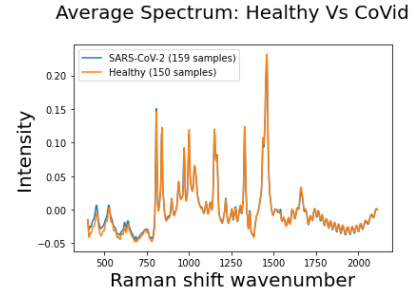
\includegraphics[width=7.0cm]{figures/Raman_average_spectra.PNG}
		%\caption{$\approx 50:50$ COVID to Healthy class ratio.}
	\end{figure}

\end{frame}

\begin{frame}{High dimensional data visualization - PCA}
%\linespread{1.3}
\begin{itemize}
    \item Over 50 percent variance explained with two principal components.
    \item No visual class separation
    %\item Dimension reduction with PCA
\end{itemize}
\begin{figure}
		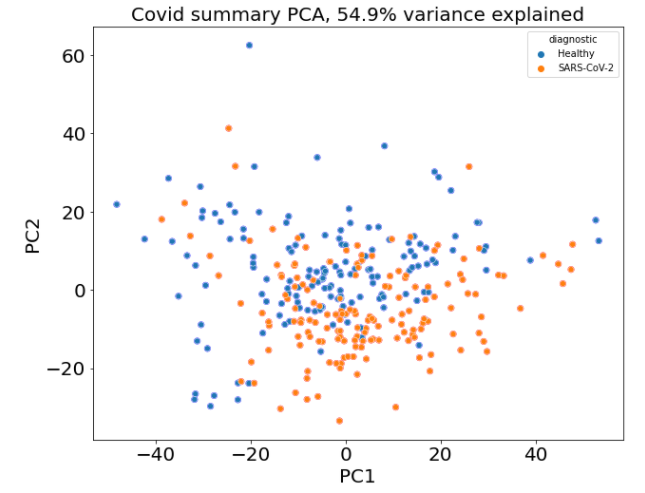
\includegraphics[width=7.0cm]{figures/pca_2_components.PNG}
		%\caption{$\approx 50:50$ COVID to Healthy class ratio.}
	\end{figure}

\end{frame}


\begin{frame}{Principal component analysis -- feature reduction}
%\linespread{1.3}
\begin{itemize}
    \item Over $90\%$ data variance explained with 15 components.
    \item Feature reduction to 15 from 900!
    %\item Dimension reduction with PCA
\end{itemize}
\begin{figure}
		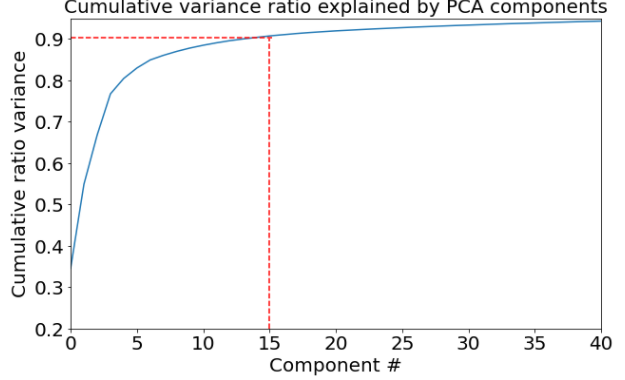
\includegraphics[width=7.0cm]{figures/pca.png}
		%\caption{$\approx 50:50$ COVID to Healthy class ratio.}
	\end{figure}

\end{frame}


%%%%%%%%%%%%%%%%%%%%%%%%%%%%%%
%%%%%%%%%%%%%%%%%%%%%%%%%%%%%%
\section{Modeling} %%%%
%%%%%%%%%%%%%%%%%%%%%%%%%%%%%%
%%%%%%%%%%%%%%%%%%%%%%%%%%%%%%

\begin{frame}{Modeling: Supervised Machine Learning}
%\linespread{1.3}
Three models considered:
%\begin{itemize}
%    \item Decision tree
%    \item Logistic regression
%    \item Random forest
%\end{itemize}
\begin{figure}
		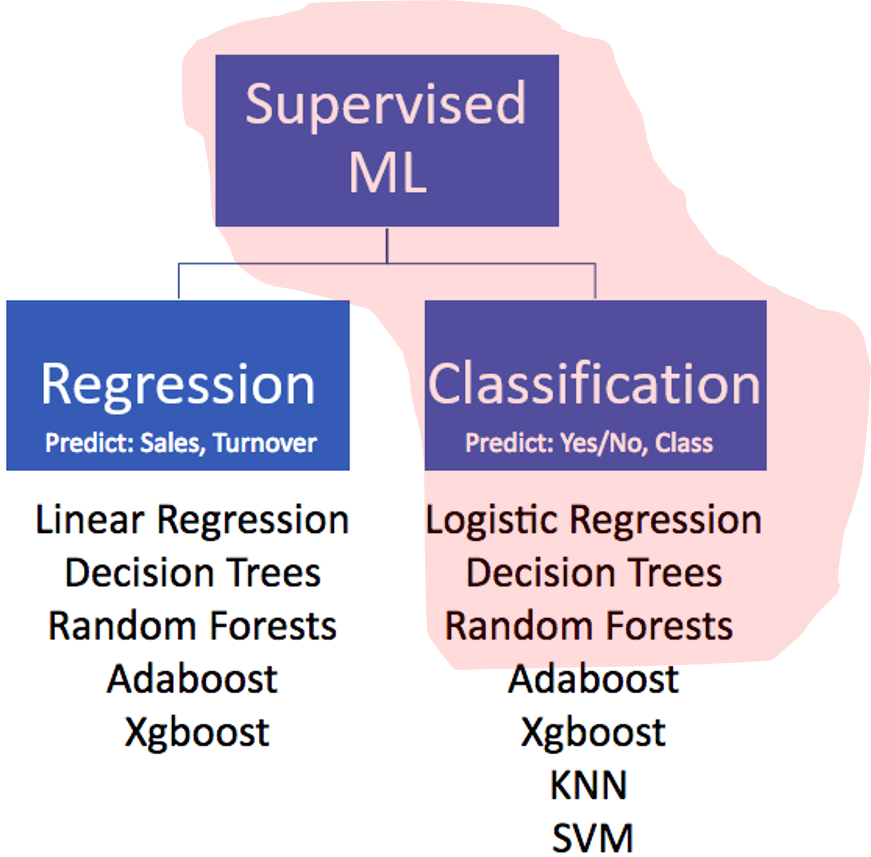
\includegraphics[width=7.0cm]{figures/ML.png}
		%\caption{$\approx 50:50$ COVID to Healthy class ratio.}
	\end{figure}
%\center{All models seem to over-fit.}
%\center{\textcolor{blue}{Need to be tested with the test split.}}
\end{frame}


\begin{frame}{Classification Report Training dataset: Logistic Regression}
%\linespread{1.3}
%Three models considered:
%\begin{itemize}
%    \item Decision tree
%    \item Logistic regression
%    \item Random forest
%\end{itemize}
\begin{figure}
		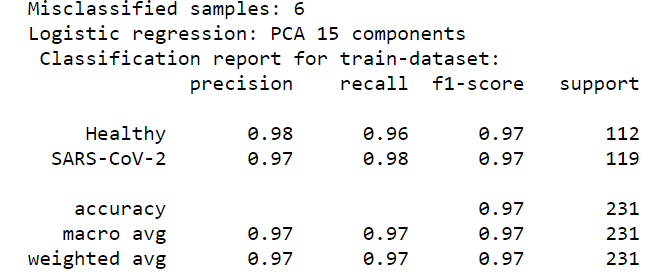
\includegraphics[width=9.0cm]{figures/log_pca_train.PNG}
		%\caption{$\approx 50:50$ COVID to Healthy class ratio.}
	\end{figure}
\center{97 percent accuracy!}
\center{\textcolor{blue}{Need to be tested with the test split.}}
\end{frame}

\begin{frame}{Classification Report Training split: Decision Tree}
%\linespread{1.3}
%Three models considered:
%\begin{itemize}
%    \item Decision tree
%    \item Logistic regression
%    \item Random forest
%\end{itemize}
\begin{figure}
		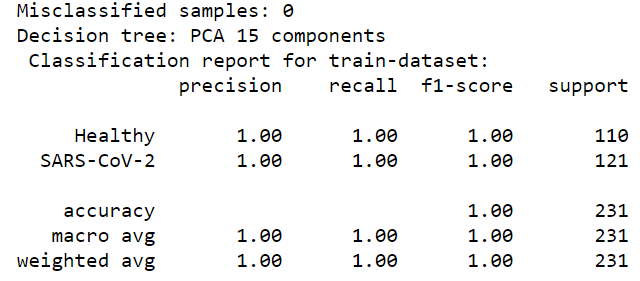
\includegraphics[width=9.0cm]{figures/dtree_pca_train.PNG}
		%\caption{$\approx 50:50$ COVID to Healthy class ratio.}
	\end{figure}
\center{100 percent accuracy! Model might be over-fitting.}
\center{\textcolor{blue}{Need to be tested with the test split.}}
\end{frame}

\begin{frame}{Classification Report Training split: Random Forest}
%\linespread{1.3}
%Three models considered:
%\begin{itemize}
%    \item Decision tree
%    \item Logistic regression
%    \item Random forest
%\end{itemize}
\begin{figure}
		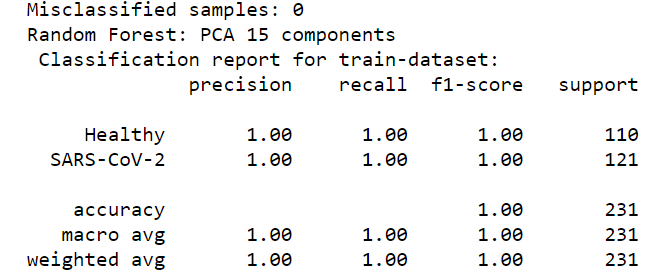
\includegraphics[width=9.0cm]{figures/forest_pca_train.PNG}
		%\caption{$\approx 50:50$ COVID to Healthy class ratio.}
	\end{figure}
\center{100 percent accuracy! Model might be over-fitting.}
\center{\textcolor{blue}{Need to be tested with the test split.}}
\end{frame}

\begin{frame}{Models Testing With Test Split}
%\linespread{1.3}
%Three models considered:
\begin{itemize}
   \item All models performed well
    \item RF and Logistic regression have highest accuracy
%    \item 
\end{itemize}
\begin{figure}
		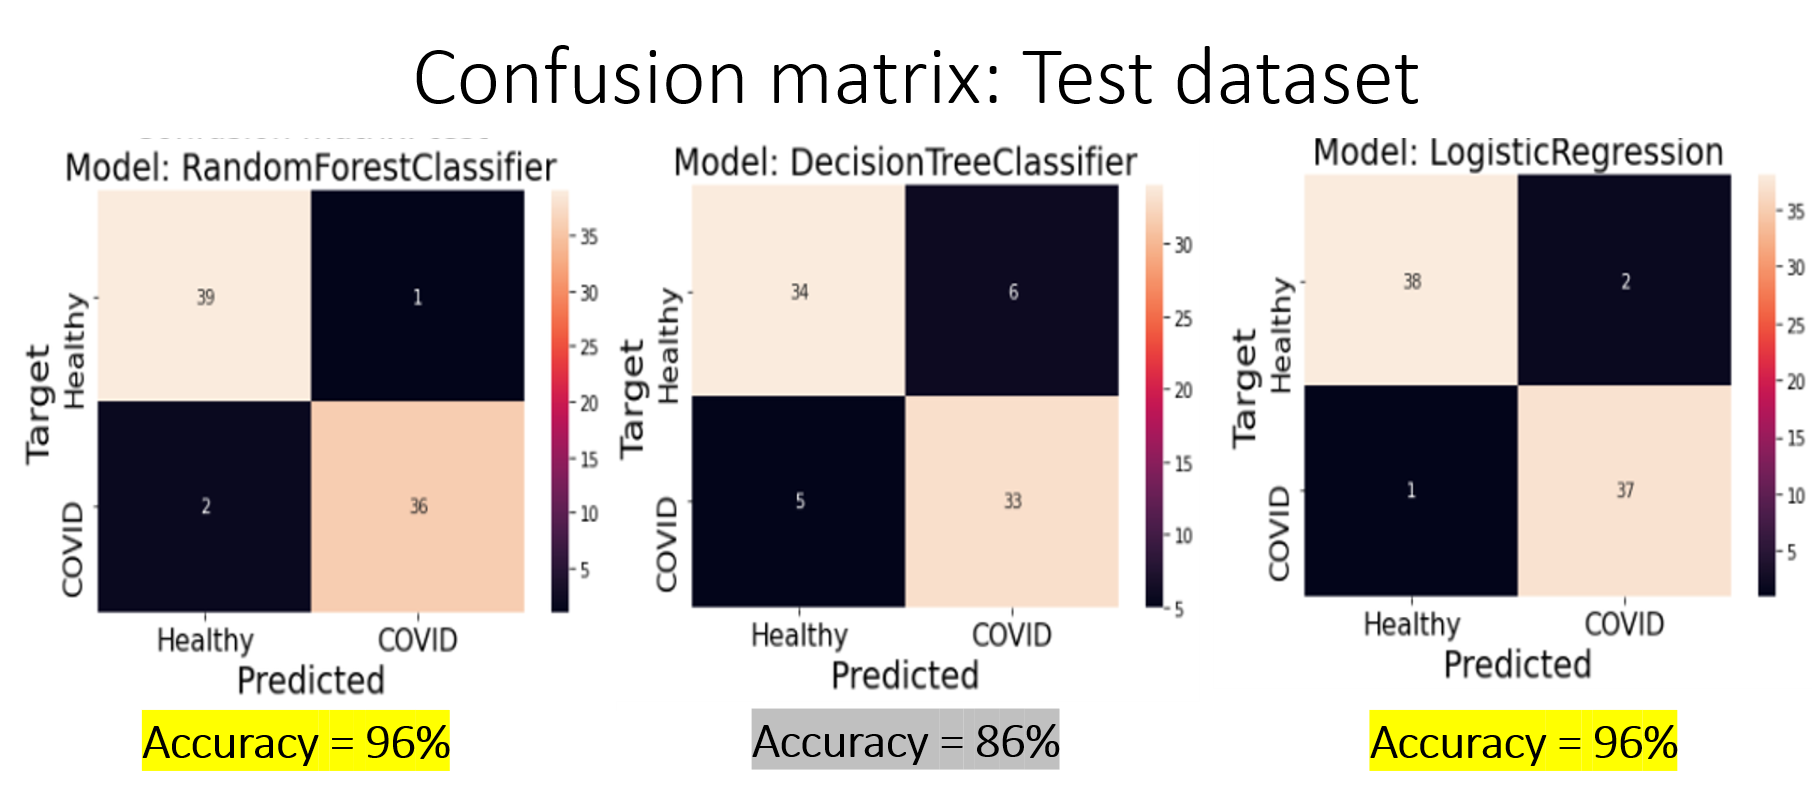
\includegraphics[width=9.0cm]{figures/cm_pca.png}
		%\caption{$\approx 50:50$ COVID to Healthy class ratio.}
	\end{figure}

\center{\textcolor{blue}{With PCA physical meaning of features is lost.}}
\center{Need to model using all features without PCA to gain physical insight on features.}
\end{frame}

\begin{frame}{Random forest classifier is the best performing model}
%\linespread{1.3}
Though all models persisted with good accuracy:
\begin{itemize}
    \item Random fores performs the best
    \item $97\%$ classification accuracy
    \item Random forest chosen for deployment
\end{itemize}
\begin{figure}
		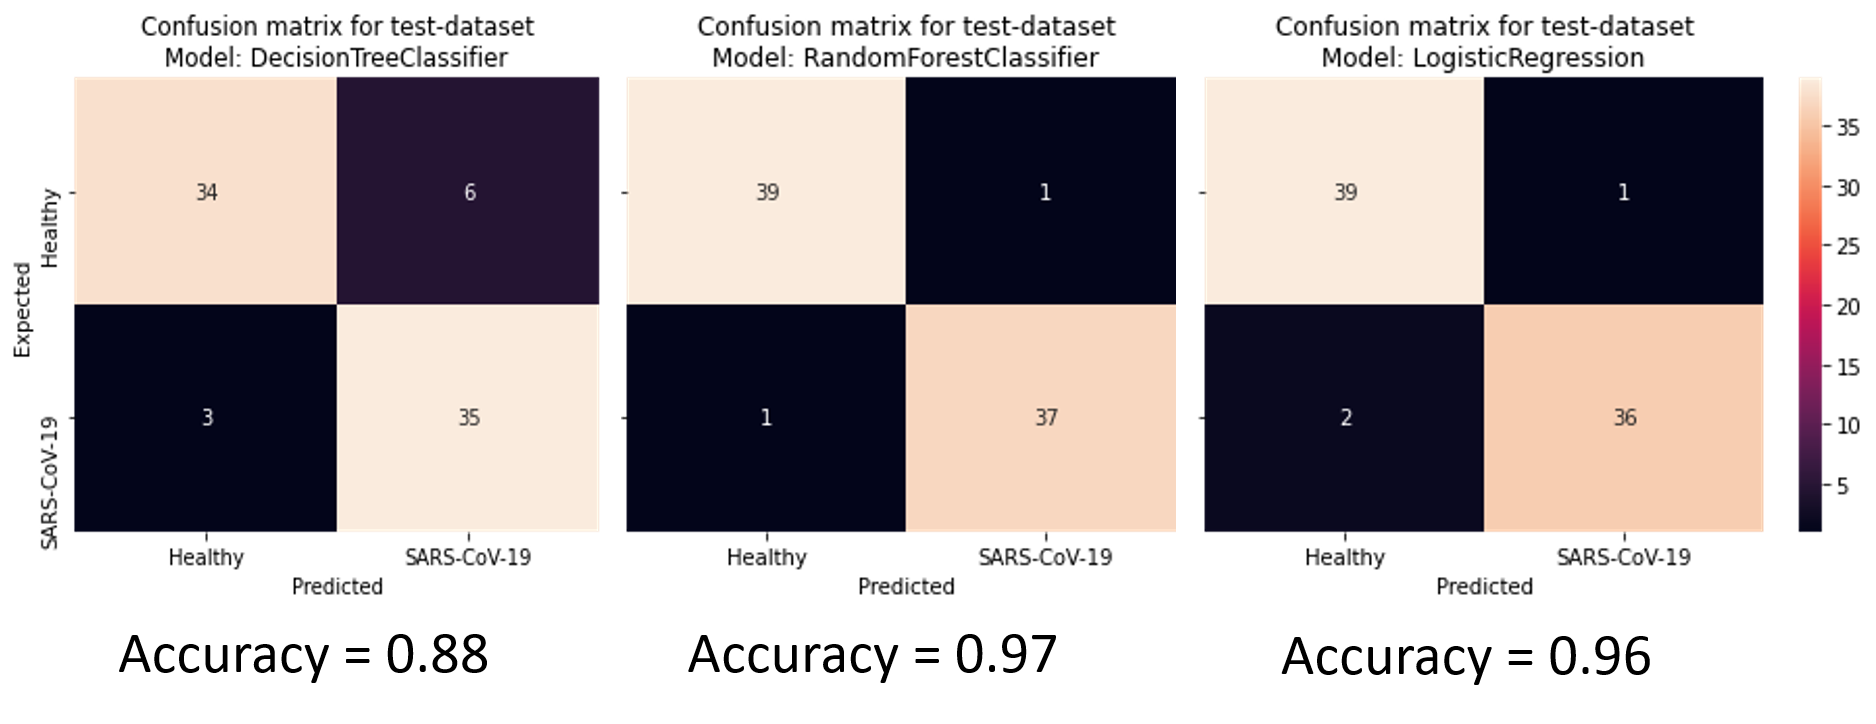
\includegraphics[width=9.0cm]{figures/c_mat.png}
		%\caption{$\approx 50:50$ COVID to Healthy class ratio.}
	\end{figure}
%\center{All models seem to over-fit.}
%\center{\textcolor{blue}{Need to be tested with the test split.}}
\end{frame}

\begin{frame}{Important features with high predictive power}
30 features out of 901 are the most important.
\vspace{0.1cm}
%\linespread{1.3}
\begin{itemize}
    \item Wavenumber in range $\left[650,870\right]$ has high predictive power
    \item feature 870 has the highest predictive power 
\end{itemize}
\begin{figure}
		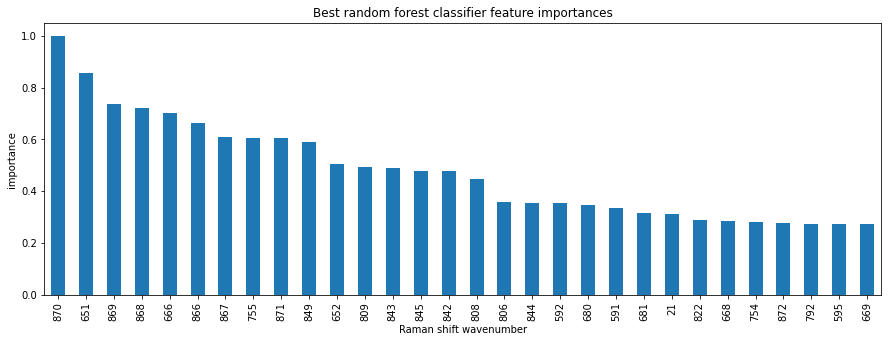
\includegraphics[width=9.0cm]{figures/predictive_features.png}
		%\caption{$\approx 50:50$ COVID to Healthy class ratio.}
	\end{figure}
%\center{All models seem to over-fit.}
%\center{\textcolor{blue}{Need to be tested with the test split.}}
\end{frame}

\begin{frame}{Important features Raman band corresponds to RNA/DNA band}

\vspace{0.1cm}
%\linespread{1.3}
\begin{itemize}
    \item Virus is an RNA/DNA protein
    \item Band $\left[700,900\right]$ is prominent for RNA/DNA
    \item Band corresponds to predicted important features
\end{itemize}
\begin{figure}
		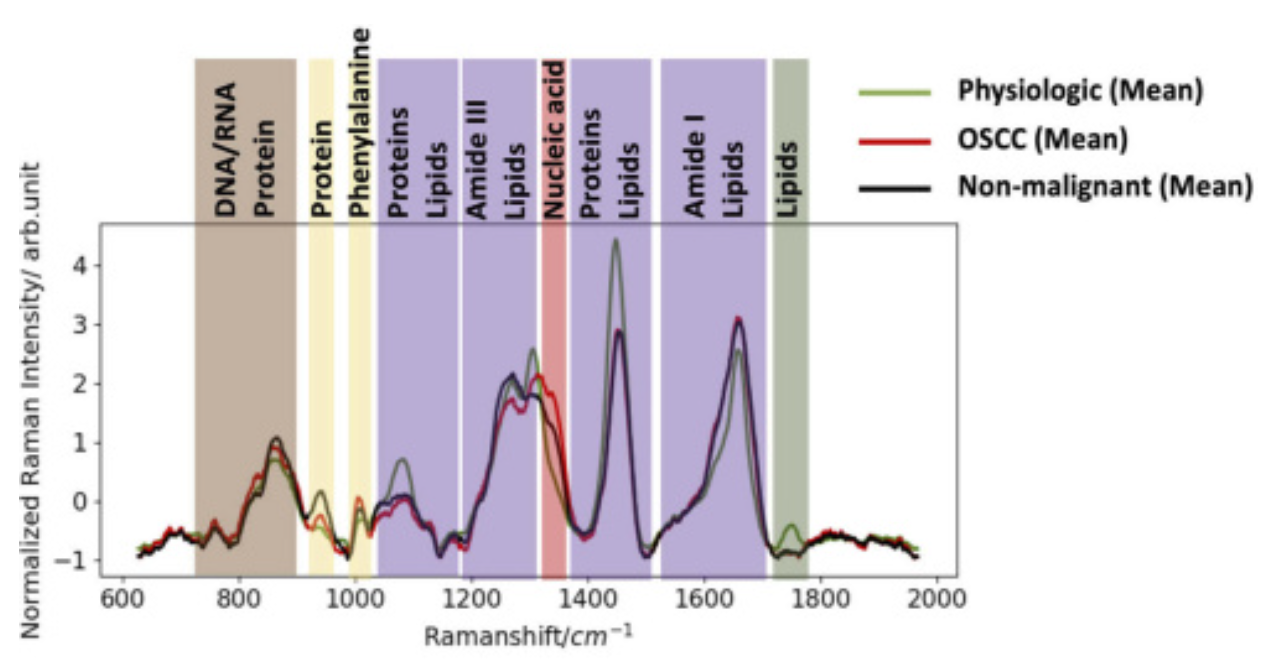
\includegraphics[width=9.0cm]{figures/virus_raman.PNG}
		%\caption{$\approx 50:50$ COVID to Healthy class ratio.}
	\end{figure}
%\center{All models seem to over-fit.}
%\center{\textcolor{blue}{Need to be tested with the test split.}}
\end{frame}

\begin{frame}{Do we need more data to enhance model performance?}
Model accuracy saturates well before the end of available data.
\vspace{0.1cm}
%\linespread{1.3}
\begin{figure}
		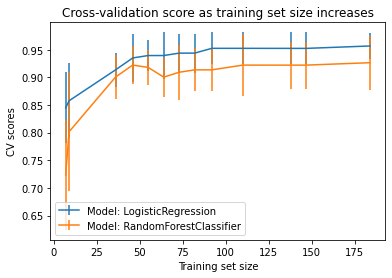
\includegraphics[width=7.0cm]{figures/cv_train_size.png}
		%\caption{$\approx 50:50$ COVID to Healthy class ratio.}
	\end{figure}
%\center{All models seem to over-fit.}
\center{\textcolor{blue}{No need for more data.}}
\end{frame}


%%%%%%%%%%%%%%%%%%%%%%%%%%%%%%
%%%%%%%%%%%%%%%%%%%%%%%%%%%%%%
\section{Summary} %%%%
%%%%%%%%%%%%%%%%%%%%%%%%%%%%%%
%%%%%%%%%%%%%%%%%%%%%%%%%%%%%%


\begin{frame}{Summary and Future Work}
\linespread{1.3}

\begin{itemize}
    \item We developed supervised machine learning models COVID detection using Raman spectroscopy data.
    \item Logistic regression, decision tree, and random forest supervised machine learning algorithms were considered.
    \item We find COVID detection using Random forest results in highest detection accuracy of 97 percent. 
    \item Future works needs to be done with covid suspect and covid survived data for more comprehensive and reliable conclusion.
    
\end{itemize}


\end{frame}


%%%%%%%%%%%%%%%%%%%%%%%%%%%%%%
%%%%%%%%%%%%%%%%%%%%%%%%%%%%%
\section{Acknowledgement} %%%%
%%%%%%%%%%%%%%%%%%%%%%%%%%%%%%
%%%%%%%%%%%%%%%%%%%%%%%%%%%%%%

\begin{frame}{Acknowledgement}
\linespread{1.3}

\center{\textbf{Springboard mentor:} Yuxuan Xin}
\center{for time generous and insightful discussions}

\end{frame}






\end{document}
